\documentclass{article}

\usepackage[left=2cm, right=2cm]{geometry}
\usepackage{hyperref}
\usepackage{graphicx}
\title{Data processing tools for dot detection (https://gitlab.com/dnadev/sdd\_dots, version 0.5)}
\author{Albertas Dvirnas}

\begin{document}
%
\maketitle
%
\iffalse
The what, the why, the how
\fi

We describe how the outputs of the two-channel fluorescence imaging experiments were processed using custom written MATLAB software. The purpose of the data processing was to detect molecules in the microscopy images of YOYO-1 channel and the positions and amount on enzymatic labels in the second channel. The pipeline can be summarized by four main steps: artifact removal, segmentation, barcode extraction and dot detection. The parameters used are summarized in table \ref{table:1}.

\begin{table}[h!]
	\centering
	\caption{{\bf List of parameters used in in sdd\_dots pipeline.}}
	\begin{tabular}{|c|c|c|}
		\hline
		Name & Value & Explanation \\
		\hline
		nmpx & 110 & Pixel size of camera in nano-meters\\
		logSigmaNm & 300 & Width of Laplacian of Gaussian filter in nano-meters\\
	  CH0 & C=0 & 	YOYO-1 channel flag\\
	  CH1 & C=1 & 	Dot channel flag\\
		widthLims & [1 Inf] & Minimum/maximum molecule width in pixels (px)\\
		lengthLims & [50 Inf] & Minimum/maximum molecule length in px\\
		minE & 2 & Margin at the edge of molecule for dot detection\\
	elim & 0.8 & Minimum molecule eccentricity\\
		ratlim & 0.4 & minimum molecule to convex hull ratio\\
		method &spline/line & molecule detection method.\\
		\hline
	\end{tabular}
	\begin{flushleft}
		All the parameters can be varied by modifying values in the GUI of the matlab script. Additional parameters are hard-coded in the script as they are changed less frequently.
	\end{flushleft}
	\label{table:1}
\end{table} 

In the first step of artifact removal, we assume that artifacts are shaped like circles and have higher intensity than that of the DNA labeled with YOYO-1. We calculate the two level image intensity threshold for the YOYO-1 image using matlab's \texttt{multithresh} implementation of Otsu and create a binary image based on the second intensity threshold. We then dilute the binary image by structuring element (a circle of $radius=5$) to make the connected components circle shaped. We then find coordinates of artifact circles of radius between $r_{Min}=12$ and $r_{Max}=23$ by using matlab's \texttt{imfindcircles}. Setting a minimum here makes sure that we don't consider single sporadic pixels as artifacts, and setting a maximum makes sure we don't consider molecules as artifacts (in case there are very few or no actual artifacts in the image).

In the second step we want to segment the YOYO-1 image into molecules and background. We filter the YOYO-1 image with a Laplacian of Gaussian (LoG) filter with $\sigma$ of logSigmaNm/pxnm using matlab's \texttt{imfilter}. After filtering with a LoG filter, edges of the molecules should appear as zero-crossings, and we binarize the image based on zero crossings using matlab's \texttt{imbinarize}. Finally we trace the exterior boundaries of objects and boundaries of holes inside the objects using matlab's \texttt{bwboundaries}. One of the objects is then assumed to be representing background pixels (we take to be the largest of the first $10$ objects detected by \texttt{bwboundaries} ). Background pixels are assgined the original intensities of these pixels in the YOYO-1 image. For the rest of the objects we check if object is intersected by an artifact (using \texttt{inpolygon}) and then calculate edge scores from the intensities of LoG image logI by summing the values of $n$ points (n depends on nmpx) from the zero crossing in the gradient direction, i.e.:
%
\begin{equation}
	edge\_score(k)= \sum_{i=1}^{N_k} \left( \sum_{d=1}^n logI(x_i-d\cdot g_{x_i},y_i-d\cdot g_{y_i}) -  \sum_{d=1}^n logI(x_i+d\cdot g_{x_i},y_i+d\cdot g_{y_i})\right)
\end{equation}
%
We then set an auto-threshold {\rm scoreThresh} on the edge scores $edge\_score$ by calculating a threshold again using Otsu. This works well if there is a lot of molecules in the image, but some care should be taken if there are very few molecules in the image. Finally unsuitable  molecules are filtered based on  {\rm scoreThresh, elim, ratlim, lengthLims, widthLims}. Binary mask matrices with the molecule positions are then saved for further steps.


To extract barcodes from molecule masks, we'll explain the procedure to fit a spline,  since line method works well only when molecules are straight. To extract the barcode from the molecule mask matrix, we first create a skeleton using matlab's \texttt{bwskel} with minimum branch length $=20$ (so that short branches would be removed). We then smoothen the data using quadratic fit method with matlab's \texttt{smooth} function. We then fit a smoothing spline using matlab's \texttt{fit} function. We then sample equidistant points along the spline and extract their intensity values using matlab's 2D interpolation function \texttt{interp2}. Sampling these points over the dots image, this gives us barcode intensity values along the molecule.

To detect dot positions along the barcode $B(i)$, we first substract the median of the background form the barcode. We then filter with a 1D LoG filter using matlab's \texttt{imfilter}. In this case it's not the zero-crossing, but the minima which gives us the locations $p_L(i)$ of the dots $i=1,2\ldots N$ along the molecule, where $N$ is the number of dots on the molecule. We estimate the peak depth along the molecule by finding the minima between ($p_L(i) \pm \sigma$) to the boundaries of the molecule. As the peak score, we take the sum over the peak and a few surrounding pixels, i.e. 
%
\begin{equation}
	dot\_score(i) = \sum_{k=-\sigma_2\ldots \sigma_2}  B(p_L(i)+k),
\end{equation}
 where $\sigma_2 = sF\cdot \sigma$, where $\sigma$ is ratio between wavelengths in the two channels (red/green).
%
Here we also calculate the auto-threshold for dot scores. Since we have estimated the intensities of background pixels before, we take the moving mean (matlab's \texttt{movmean}) over the background pixels, to get the same averaging statistics as for the dot scores, since there we average over $=-\sigma_2\ldots \sigma_2$. The threshold is then taken to be $n$ times standard deviation of the averaged background pixels minum the background median. We take $n=2$ sigma rule in order not too be too strict when detecting dots, since 1) background intensity could be over-estimated if some signal pixels are included in background calculation, and 2) even though we're using spline detection, the detected curve might not pass through the "center" of the dot, thus resulting in lower score. The detected molecules are the visualized, and the results saved in an output txt file.

\begin{figure}
		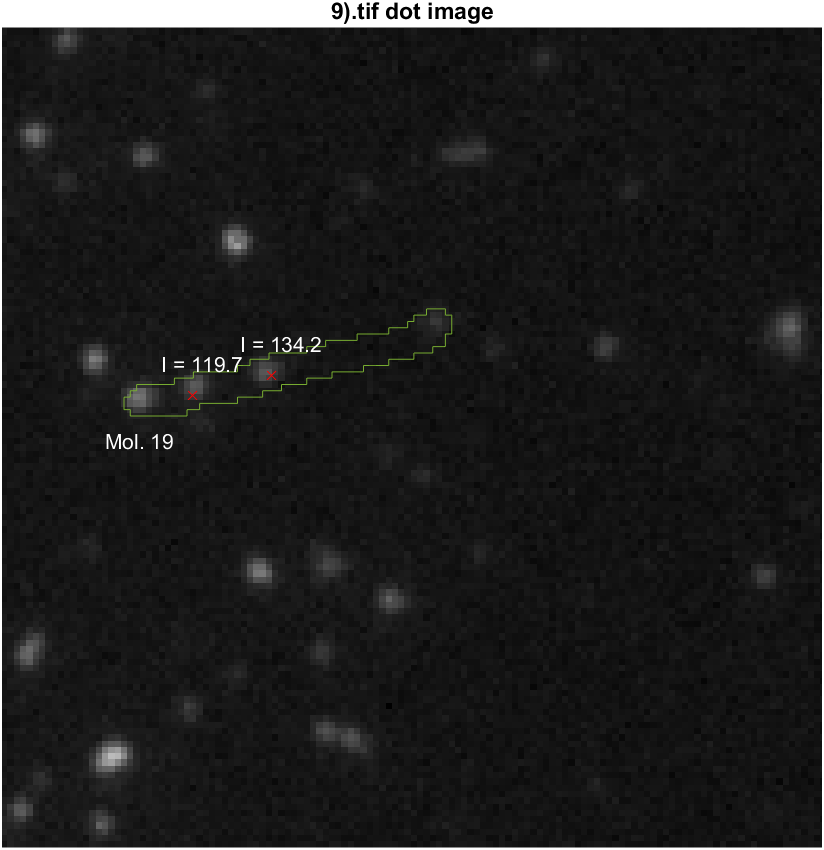
\includegraphics{image.png}
		\caption{{\bf Example of visual output}. A molecule is given an index (in this case Mol.19), detected dot positions are labelled by a red cross, and dot scores are printed out above.}
\end{figure}


\iffalse
If include bibliography
\begin{thebibliography}{10}
	\bibitem{} 
\end{thebibliography}
	\fi
\end{document}